\chapter{Value-sensitive rejector}
\label{ch:rejector}
As concluded in chapter \ref{ch:related-work}, there is a need for \textit{value-sensitive} metrics for measuring the performance of ML models, especially for social-technical applications such as hate speech detection.
%
We also concluded that manual human moderation is the most effective and that most automatic hate speech detection methods do not perform well on unseen data.
%
Therefore, in this project, we focus on rejecting ML predictions in a value-sensitive manner.
%
We do this by taking the values of TP, TN, FP, FN, and rejected predictions into account.
%
% Correct predictions (TP and TN) result in positive value (gains), while incorrect (FP and FN) and rejected predictions result in negative value (costs).
%
Chapter \ref{ch:survey} will explain how we assess these values.
%
We assume that we know these values for the remaining part of this chapter.
%

%
In this chapter, we explain how we create a value-sensitive dependent rejector by introducing a value-sensitive confidence metric that measures the total value of an ML model with a reject option.
%
In \ref{sec:value-metric}, we explain how we construct the confidence metric.
%
In \ref{sec:overview-rejector}, we provide an overview of how we use the value-sensitive rejector, and in \ref{sec:state-of-the-art}, we discuss how we apply the rejector to some state-of-the-art hate speech classification models.

\section{Value-sensitive metric}
\label{sec:value-metric}
The idea of rejecting ML predictions using a threshold is that for some threshold value $\tau$ in the range $[0, 1]$, we accept all predictions with confidence values greater than or equal to $\tau$ and reject all predictions with confidence values below $\tau$.
%
We use a confidence metric to find the optimal rejection threshold.
%
Here, we introduce our confidence metric as the value function $V(\tau)$ that measures the total value of an ML model and rejection threshold $\tau$.
%
We can determine the optimal rejection threshold by finding the $\tau$ value for which $V(\tau)$ is the maximum.
%
The value of $V(\tau)$ depends on the values of TP, TN, FP, FN, and rejected predictions, and we calculate it for a set of predictions with their corresponding confidence values and actual labels.
%
We denote the values of TP, TN, FP, FN, and rejected predictions as $V_{tp}$, $V_{tn}$, $V_{fp}$, $V_{fn}$, and $V_r$, respectively.
%
We can derive the subsets of TP, TN, FP, and FN predictions from the complete set of predictions and their predicted and actual labels
%

%
We should be free to use any value for $V_{tp}$, $V_{tn}$, $V_{fp}$, $V_{fn}$, and $V_r$ since we do not know which values will come from the survey study in chapter \ref{ch:survey}.
%
However, for constructing our metric, we can define several conditions if we assume that $V_{tp}$ and $V_{tn}$ are gains and, therefore, positive values and $V_{fp}$, $V_{fn}$, and $V_{r}$ are costs and, therefore, negative values.
%
For each $\tau$ value in $[0, 1]$, we would like to know whether the model with the reject option is more effective (increased $V(\tau)$) or less effective (decreased $V(\tau)$ value).
%

\pagebreak

%
\begin{flushleft}
    We define the following conditions:
\end{flushleft}
\begin{enumerate}
    \item The value of incorrect predictions should be lower than that of rejected predictions. Otherwise, adopting the reject option serves no purpose.
    \item Correct accepted predictions should increase the value of $V(\tau)$, while incorrect accepted predictions should decrease the value of $V(\tau)$.
    \item Correct rejected predictions should decrease the value of $V(\tau)$, while incorrect rejected predictions should increase the value of $V(\tau)$.
\end{enumerate}
%
We can formulate the first condition as follows:
% 
\begin{align}
    \label{for:value-condition}
    \frac{V_{fp} + V_{fn}}{2} < V_r,
\end{align}
%
We can convert the latter two conditions into the following equations:
\begin{subequations}
    \label{for:conditions}
    \begin{align}
        \frac{\partial V}{\partial F_{tp}} + \frac{\partial V}{\partial F_{tn}} > 0, &  &
        \frac{\partial V}{\partial F^r_{tp}} + \frac{\partial V}{\partial F^r_{tn}} < 0, \label{for:conditions-tp-tn} \\
        \frac{\partial V}{\partial F_{fp}} + \frac{\partial V}{\partial F_{fn}} < 0, &  &
        \frac{\partial V}{\partial F^r_{fp}} + \frac{\partial V}{\partial F^r_{fn}} > 0, \label{for:conditions-fp-fn}
    \end{align}
\end{subequations}
%
where $F_p$ and $F_p^r$ are the fractions of accepted and rejected predictions, respectively and $p \in [tp, tn, fp, fn]$.
%
% All conditions include greater/smaller than or equal to operators, since we want to allow the values of $V_{tp}$, $V_{tn}$, $V_{fp}$, $V_{fn}$, and $V_{r}$ to be equal to zero.
%
We create a linear $V(\tau)$ function and assume that the values $V_t$ are known constants.
%
Subsequently, we can formulate $V(\tau)$ as:
\begin{align}
    \label{for:V}
    V(\tau) = \sum_{p} (V_p - V_r)F_p(\tau) + \sum_{p} (V_r - V_p)F^r_{p}(\tau),
\end{align}
%
where $p \in [tp, tn, fp, fn]$ and where $F_p(\tau)$ and $F_p^r(\tau)$ are the fractions of accepted and rejected predictions dependent on the rejection threshold $\tau$.
%
Conditions \ref{for:conditions-tp-tn} are satisfied by default since we assume that $V_{tp}$ and $V_{tn}$ are positive and $V_r$ is negative.
%
Conditions \ref{for:conditions-fp-fn} are satisfied since we assume that $V_{fp}$, $V_{fn}$, and $V_r$ are negative, and when condition \ref{for:value-condition} holds.
% 
We can retrieve the $F_p$ and the $F_p^r$ values by computing the integrals over the probability density functions (PDF) of the confidence values (denoted as $x$) of the predictions with type $p$.
%
We denote $F_p$ by taking the integral over the interval $[\tau, 1]$, and $F_p^r$ by taking the integral over the interval $[0, \tau]$:
%
\begin{align}
    \label{for:R}
    \begin{aligned}
        F_{p}(\tau) = \int_\tau^1 D_p(x)dx & \quad & F_p^r(\tau) = \int_0^\tau D_p(x)dx,
    \end{aligned}
\end{align}
%
where $D_p$ is the PDF of all predictions of type $p$.
%
By inserting the integrals from \ref{for:R} into \ref{for:V}, we get our final value function:
%
\begin{align}
    \label{for:final-V}
    V(\tau) = \sum_p (V_p - V_r)\int_\tau^1 D_p(x)dx + \sum_p (V_r - V_p)\int_0^\tau D_p(x)dx
\end{align}
%
We can now use \ref{for:final-V} to calculate the total value of an  ML model for all thresholds $\tau \in [0, 1]$.
%
The theoretical optimal rejection threshold is equal to the $\tau$ value for which we achieve the maximum value of $V(\tau)$.
%
We can find the optimal rejection threshold $\tau_O$ using the following formulation:
%
\begin{align}
    \label{for:optimal-threshold}
    \tau_O \text{ where } V(\tau_O) = \max \{V(\tau): \tau \in \mathbb{R} \wedge 0 \leq \tau \leq 1 \}
\end{align}

\section{Overview of the value-sensitive rejector}
\label{sec:overview-rejector}
This section provides an overview of how we use our value-sensitive rejector.
%
We distinguish a training phase and a deployment phase of the rejector.
%
In this project, we mainly focus on the training phase since we do not apply the rejector in the wild.
%
Figures \ref{fig:training} and \ref{fig:deployment} visualize how we train the rejector and how we can use it in deployment to accept or reject predictions, respectively.
%
In figure \ref{fig:training}, we show the training phase of the rejector.
%
In this phase, we use our value-sensitive metric from section \ref{sec:value-metric} to calculate the optimal rejection threshold $\tau_O$.
%
We use the following inputs in this calculation: the values from the crowdsourced survey and a set of predictions that consist of the confidence values and the predicted and actual labels.
%
Figure \ref{fig:deployment} shows how we can apply the trained rejector to unseen data in deployment
%
We accept all predictions for which the confidence value $c$ is greater than or equal to the optimal rejection threshold $\tau_O$ and, otherwise, reject them so that a human moderator handles the prediction.
%
\begin{figure}
    \centering
    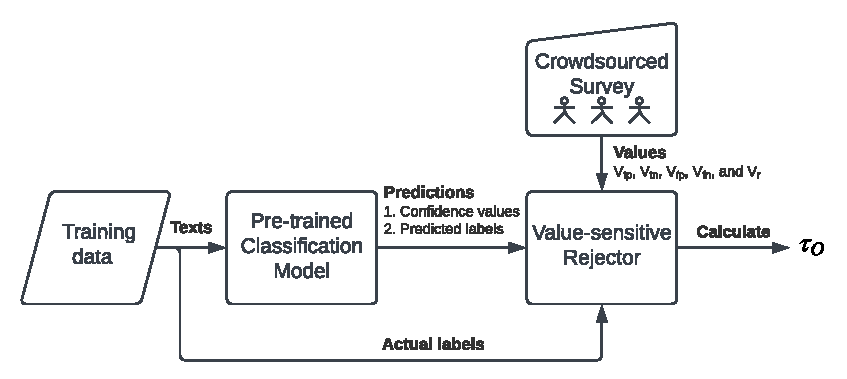
\includegraphics[scale=.75]{Figures/training.pdf}
    \caption{\textbf{Training phase:} flow diagram that visualizes how the value-sensitive rejector calculates the optimal rejection threshold $\tau_O$.}
    \label{fig:training}
\end{figure}
%
\begin{figure}
    \centering
    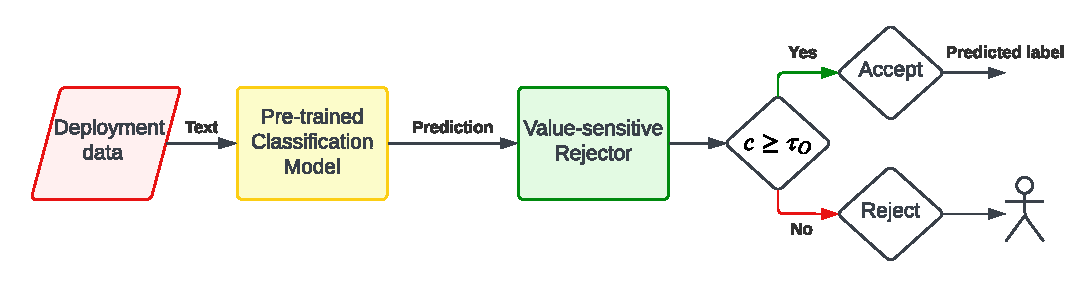
\includegraphics[scale=.75]{Figures/deployment.pdf}
    \caption{\textbf{Deployment phase:} flow diagram that visualizes how the value-sensitive rejector uses the optimal rejection threshold $\tau_O$ and the prediction confidence $c$ to determine when to accept or reject a prediction from unseen data in deployment.}
    \label{fig:deployment}
\end{figure}

\section{State-of-the-art}
\label{sec:state-of-the-art}
This section will explain how we apply the value-sensitive rejector to some of the state-of-the-art automatic hate speech detection models.
%
In this experiment, we aim to find out three things.
%
First, we want to determine how the value-sensitive rejector behaves on different models and datasets.
%
Second, we want to know whether value-sensitive rejection can benefit hate speech detection.
%
Finally, we compare the values of our value-sensitive metric to the values of machine metrics such as accuracy and check whether they give different results.
%

\subsection{Models}
We experiment with three different hate speech detection models based on the findings from related work in section \ref{sec:related-work-detection-algorithms}.
%
The first model is a traditional ML model.
%
We implement the Logistich Regression (LR) model with Character N-gram from \citet{waseem2016hateful} since this model achieved the best performance compared to other traditional ML models \citep{davidson2017automated}.
%
We select the second model, a DL model, based on the findings from \citet{agrawal2018deep, badjatiya2017deep}.
%
We choose a Convolutional Neural Network (CNN) model initialized with random word embeddings since both studies found that this configuration provides state-of-the-art classification performance.
%
We implement the CNN model based on the work of \citep{agrawal2018deep}.
%
Finally, our third model is a transformer model, given its recent popularity in the NLP domain.
%
We use the DistilBERT model since it is faster to train and smaller than BERT models while achieving similar performance \citep{sanh2019distilbert}.
%g
We implement all models in Python.
%
We implement the LR model with scikit-learn\footnote{\url{https://scikit-learn.org/}}, the CNN model with TensorFlow\footnote{\url{https://www.tensorflow.org/}}, and the DistilBERT model with a combination of Hugging Face\footnote{\url{https://huggingface.co/}} and PyTorch\footnote{\url{https://pytorch.org/}}.
%
We use Google Colab\footnote{\url{https://colab.research.google.com/}} to train all models.
%

\subsection{Hyperparameter optimization}
We perform hyperparameter optimization on all three models.
%
For the CNN model, we apply random search to optimize the values of the learning rate, batch size, and the number of epochs.
%
For the DistilBERT model, we apply Population Based Training (PBT) \citep{jaderberg2017population} implemented in Tune \citep{liaw2018tune}, to optimize the values of the batch size, learning rate, and the number of epochs since Tune.
%
PBT combines random search and hand tuning by discovering potentially optimal hyperparameter values along the way to reduce optimization time \citep{jaderberg2017population}.
%
For the LR model, we use the LogisticRegressionCV model from scikit-learn that automatically optimizes the C value (inverse of regularization strength) of the LR model.

\subsection{Calibration}
The problem with most neural network models is that they are often not calibrated \citep{guo2017calibration,sayin2021science}.
%
We define calibrated models as models where the confidence values of the predictions are equal to the probabilities that the predicted labels are correct.
%
However, most neural networks tend to be sensitive to producing both low- and high-confident errors \citep{guo2017calibration, sayin2021science}.
%
A well-calibrated model that achieves a low accuracy score can still be valuable since we can reject all low-confident incorrect predictions and only accept the high-confident correct predictions \citep{sayin2021science}.
%
In our project, we aim to have calibrated models since calculating the optimal rejection threshold depends on the confidence values of the predictions.
%

%
\citet{guo2017calibration} experimented with different calibration methods.
%
They evaluated the results using the expected calibration error (ECE), which measures the difference between the expected confidence and accuracy \citep{guo2017calibration}.
%
They found that the temperature scaling method is the most effective.
%
In temperature scaling, we divide the model's output logits with a temperature value of $T$ to soften the probabilities of the final softmax function in the model's architecture \citep{guo2017calibration}.
%
This $T$ value is initially set to $1$ and optimized by minimizing the negative log likelihood \citep{guo2017calibration}.
%
Please note that temperature scaling does not change the model's accuracy but only rescales the distribution of the confidence values \citep{guo2017calibration}.
%

%
As we experiment with two neural networks (DistilBERT and CNN), we apply temperature scaling to calibrate both models.
%
However, calibration with temperature scaling does not guarantee perfect calibration.
%
Therefore, high-confident incorrect predictions and low-confident correct predictions can still occur after calibration.
%
Nevertheless, it is still valuable to calibrate the models since it also benefits human interpretation of the confidence values and, therefore, the interpretation of the optimal rejection threshold.
%

%
The Logistic Regression model is well-calibrated by default since, under the hood, it optimizes the log-loss function, which measures the difference between predicted confidence values and the actual labels.
%
Therefore, we do not have to apply temperature scaling to the Logistic Regression model.

\subsection{Datasets}
We train all models on the \citet{waseem2016hateful} dataset consisting of 16K tweets labelled racist, sexist, or neutral.
%
We converted the 'racist' and 'sexist' labels to 'hate' labels to create a binary classification setting.
%
Furthermore, we split the dataset into a train and test dataset according to an 80:20 ratio.
%
For the CNN and the DistilBERT models, we split the training set up into a training set and a validation set according to a 75:25 ratio.
%
We use this validation set to calibrate the trained models by finding the optimal $T$ value for the temperature scaling method.
%
We preprocess the data by tokenizing all URLs, user mentions, and emojis since these do not contain any valuable information.
%
We split all hashtags up into separate words using the WordSegment\footnote{\url{https://pypi.org/project/wordsegment/}} library.
%
The remaining parts of the preprocessing, such as removing whitespaces and stop words or the tokenization process, are dedicated to the different frameworks we use per model.
%

%
We apply the value-sensitive rejector to two test datasets: the \emph{seen} dataset and the \textit{unseen} dataset.
%
The seen dataset is the test set from the \citet{waseem2016hateful} dataset.
%
The unseen dataset is a test set from the \citet{basile2019semeval} dataset that consists of 10K English tweets labelled as either hateful (against immigrants or women) or not hateful.
%
We use the unseen dataset to simulate how the models would perform in a realistic use-case when a model is trained on one dataset and applied to a different dataset.
%

%
We want to study the effect of bias and how this affects the results when using our value-sensitive metric for evaluating the models with a reject option.
%
We expect that the accuracy of the predictions on the unseen dataset is significantly lower than on the seen dataset, similar to the findings of related studies: \citet{grondahl2018all, arango2019hate}.
%
Therefore, we also expect that the output value of our value-sensitive metric for the unseen dataset will be lower and that the optimal rejection threshold will be higher (meaning that we need to reject more predictions).
%

\subsection{Probability density functions}
Since our value-sensitive rejector depends on the PDFs of the confidence values of the TP, TN, FP, and FN predictions, we need to empirically estimate these PDFs as we do not know the actual underlying distributions.
%
We use the kernel density estimation (KDE) method provided by Statsmodels\footnote{\url{https://www.statsmodels.org/}} for estimating these PDFs.
%
With KDE, we estimate the PDF by weighing each measured confidence value from a set of predictions using a kernel function, a gaussian density function since it is the most commonly used, for each possible confidence value in the range $[0, 1]$.
%
If there are many predictions with a confidence value around $0.8$, then the KDE estimate will be higher around that point.
%
The kernel function used in the KDE method also depends on a bandwidth (smoothness) value.
%
A small bandwidth value results in an estimated PDF with much variance, while a high bandwidth value results in an estimated PDF with much bias.
%
We use maximum likelihood cross-validation to find the optimal bandwidth value.

\subsection{Application of the value-sensitive rejector}
\label{sec:rejector-application}
We apply the training phase of the value-sensitive rejector (refer to figure \ref{fig:training}) to all three models for both the seen and the unseen datasets.
%
Therefore, we use our metric from section \ref{sec:value-metric} to calculate the total value $V(\tau)$ (formula \ref{for:final-V}) at all possible rejection thresholds ($\tau$) for all different setups.
%
We determine the optimal rejection threshold $\tau_O$ using the formulation from \ref{for:optimal-threshold}.
%
Since we have a binary classification setting (hate or not hate), all confidence values will always be greater than or equal to $0.5$.
%
So if $\tau \in [0.0, 0.5]$, we accept all predictions and if $\tau = 1.0$, we reject all predictions.
%
Therefore, we only calculate the total value of all predictions for the range $\tau \in [0.5, 1.0]$.
%

%
The first goal is to check the rejector's behaviour on different models and datasets.
%
We can analyze this by plotting $V(\tau)$ for the range $\tau \in [0.5, 1.0]$, measuring the rejection rate (RR, percentage of rejected predictions), and measuring the accuracy of the accepted predictions.
%
The second goal is determining whether the rejector can enhance hate speech detection.
%
If the total value of a model for some optimal rejection threshold ($0.5 < \tau_O < 1.0$) is positive, then we know that the reject option can be beneficial for that specific model.
%
The final goal is to compare the value-sensitive metric to machine metrics such as accuracy.
%
We accomplish this by comparing the $V(\tau_O)$ values and the accuracies of all models.


